\documentclass[12pt,twoside]{article}
\usepackage{amsmath}
\usepackage{amssymb}
\usepackage{graphicx}
\usepackage{algorithm}
\usepackage{algorithmicx}
\usepackage{algpseudocode}
\usepackage{booktabs}
\usepackage{tabularx}
\usepackage{geometry}
\usepackage{datetime}
\usepackage{caption}
\usepackage{titlesec}
\usepackage[titletoc]{appendix}
\usepackage{rotating}
\usepackage{csquotes}

\renewcommand*\appendixpagename{\Large Appendices}

% SET MARGINS
\geometry{
top = 1.0in,
bottom = 1.0in,
inner = 1.0in,
outer = 1.5in
}
\begin{document}
\title{An Investigation of Genetics-Based Machine Learning as Applied to Global Crop Yields \\
\quad \\
\large An Honors Paper for the Department of Computer Science}
\author{By William A. H. Gantt IV}
\date{}
\maketitle
\vfill
\begin{center}
Bowdoin College, 2017

\copyright{ William A. H. Gantt IV }
\end{center}
\clearpage
\tableofcontents
\listofalgorithms
\listoffigures
\listoftables
\clearpage
\section{Introduction}

% What is the problem that your project is trying to address?
As Earth's population continues to grow and as the effects of climate change intensify, it is critical that we better understand the environmental and economic factors that affect agricultural output around the world. While rising temperatures may benefit certain crops in the short term, extreme weather and higher levels of atmospheric $\text{CO}_2$ will, if left unchecked, have disastrous consequences for water supply, soil fertility, and, consequently, for crop yields. \cite{us_epa_climate_2017}. Moreover, the United Nations Department of Economic and Social Affairs predicts that the world population will reach 9.7 billion by 2050 and 11.2 billion by the end of the century \cite{noauthor_world_2015}.

% How do you plan to address it?
These forecasts demand prudent planning, which in turn requires that we be able to discern trends in agricultural data. To that end, I have designed and written a learning classifier system (LCS)---a powerful and versatile tool  for data mining---and have applied it to data collected by Erik Nelson in order to probe the relationships between various agricultural inputs and changes in crop yields.
This paper presents the preliminary results of my investigations. It does not aim to provide any economic or environmental explanation for those results, nor does it offer policy suggestions. Indeed, I discourage the reader from drawing from my findings any inferences about what measures we ought to be taking. Such conclusions require more data and broader, more thorough analysis than I am able to give.

% Outline of rest of paper
The following section gives a brief overview of genetics-based machine learning (GBML) and LCSs, and of the research done by Nelson and Congdon that gave rise to this project \cite{nelson_measuring_2016}. Section 3 provides a thorough description of the system design of my own LCS. Section 4 details the experiments conducted and the results. Section 5 offers some concluding remarks and suggests directions for future work. Raw data and additional information are contained in the appendices.

\section{Background}

In this section, I provide some context for my project. First, I introduce the GBML paradigm and consider the place of LCSs within it. Next, I give a general overview of LCSs and their basic structure. I then discuss a few important developments in the history of LCSs for supervised learning, and conclude by talking specifically about the earlier work of Nelson and Congdon \cite{nelson_measuring_2016}.

\subsection{Genetics-Based Machine Learning}

GBML is a machine learning approach based on evolutionary computation. Briefly, evolutionary computation comprises a set of optimization algorithms that evolve populations of candidate solutions to a particular problem through a process inspired by biological evolution. Many of the most interesting and important problems in machine learning have large and noisy search spaces, and it is in such contexts that techniques from evolutionary computation have proved particularly effective.

The precise relationships between various GBML-related terms and concepts have changed over the years, and usage in the community is often loose. GBML, once taken to refer exclusively to LCSs, is now considered a broader term that encompasses a number of other algorithms, including genetic programming, evolutionary ensembles, evolutionary neural networks, and genetic fuzzy systems \cite{kovacs_genetics-based_2012}. For the purposes of this paper, it is important only to recognize that LCSs exist within a larger machine learning problem-solving framework.

\subsection{What is a Learning Classifier System?}

\subsubsection{Structure}

Introduced by John Holland in 1975, LCSs are GBML algorithms that evolve a population of rules\footnote{Rules are also frequently referred to as ``classifiers.'' To maintain a clear distinction between individual \emph{classifiers} and the \emph{classifier systems} that comprise them, I use the term ``rule'' exclusively to denote the former, and ``LCS'' to denote the latter.} \cite{holland_adaptation_1975}. Each rule consists of a condition that indicates when the rule applies, as well as an action to take if the condition's criteria are met. As LCSs have applications to a variety of learning problems, the function of the rules depends largely on the task. With supervised learning problems, rules attempt to categorize a set of training examples by mapping the features of those examples to particular classes. In these cases, a rule's condition describes the features of the examples to which it applies, and the action specifies the class to be assigned to examples matching the condition. Problems in reinforcement learning, by contrast, often involve determining the best action for an agent to take in response to inputs or stimuli from an environment. Here, a rule's condition describes a set of inputs and its action determines how the agent should react given those inputs.

Regardless of the types of problems to which they are applied, all LCSs share certain basic structures and mechanisms. Holmes et al. have identified four such components  \cite{holmes_learning_2002}, but their model is more characteristic of LCSs used in reinforcement learning than those used in supervised learning. I suggest a slight modification of that model that covers both:
\begin{enumerate}
\item \emph{Population.} All LCSs have a population of rules. Although some systems allow for the growth or reduction of the population, there is typically a limit on the maximum number of rules it may contain.
\item \emph{Learning.} An LCS must have a means of coercing its population toward rules that generate good actions or accurate classifications. Numerous methods have been used for this purpose and they tend to vary based on the kind of learning. Many early LCSs designed for reinforcement learning used the bucket brigade algorithm \cite{holland_properties_1985}, while more contemporary systems often rely on Q-learning \cite{c._j._c._h._learning_1989, orriols-puig_fuzzy-ucs:_2009} or Q-learning-inspired algorithms. For supervised learning tasks, other systems have used genetic algorithms (GAs) exclusively \cite{llora_towards_2007}. Still others have used different approaches, including ensemble learning \cite{gao_learning_2005} and bayesian methods \cite{hai_h._dam_bcs:_2006}.
\item \emph{Discovery.} An LCS must also have mechanisms for generating new rules. For that purpose, a vast majority of systems employ GAs, which provide two useful operations: crossover and mutation. Crossover produces two ``offspring'' rules from two existing ``parent'' rules, and mutation alters some of the attribute values of the offspring. Many LCSs employ additional operators such as the \emph{covering} operator, which creates a new rule when there are none that match the current input, and which has been widely used \cite{orriols-puig_fuzzy-ucs:_2009, wilson_classifier_1995, bernado-mansilla_accuracy-based_2003}. \emph{Specify}, a second popular operator, proposed by Pier Lanzi,  attempts to counteract the over-generalization of rules by specifying the attribute values of a rule according to a particular input \cite{lanzi_study_1997}. 
\item \emph{Classification or Action Selection.} Finally, an LCS must have some procedure for deciding what action to take or how to classify a particular example. In the typical case, the action or classification is selected based on the actions recommended by the rules in the \emph{match set}---the set of rules matching a particular input. One possibility is simply to choose the action of the fittest rule in the match set. Another is to conduct a weighted vote of all the rules in the set, where each rule casts a ``vote'' for its action, weighted by its fitness. The selected action, then, is the one receiving the greatest number of points. Some systems have also incorporated random action selection alongside one of the first two methods \cite{wilson_classifier_1995}.
\end{enumerate}

At the broadest level, these are the modules that feature in all LCSs. There is, of course, substantial variation between implementations, which is to be expected of a paradigm with applications as diverse as those of the LCS algorithm.

\subsubsection{Genetic Algorithms}

As GAs constitute such a critical component of LCSs, they merit at least a short overview. GAs evolve populations of candidate solutions to a problem by a process modeled after biological evolution. In a traditional implementation, individuals are represented as bit strings, where each index in a string corresponds to a particular property of the solution and a 1 or a 0 at that index indicates the presence or absence of the property, respectively. In LCSs, a third character (a ``don't care'' value, denoted by ``\#'') is often used to indicate that the property is not relevant for a given rule. In principle, solutions may take any form, and GA variants have been developed to accommodate structures of different kinds, including objects \cite{keijzer_evolving_2001}. The canonical GA works as follows:
\begin{enumerate}
\item \emph{Initialization.} Generate a random population of candidate solutions.
\item \emph{Evaluation.} Evaluate the fitness of each individual according to some fitness function.
\item \emph{Selection.} Select $n$ individuals from the population to reproduce. The probability that a given individual will be selected is usually proportional to its fitness.
\item \emph{Crossover.} Randomly pair the $n$ selected individuals. For each pair, combine the bits of one member of the pair with those of the other (e.g. via one-point crossover) to produce two new solutions (``offspring'').
\item \emph{Mutation.} Flip some number of the bits in each offspring with probability $p$.
\item \emph{Replacement.} Replace the $n$ least-fit members of the original population with the offspring created in (5). Optionally, some number of the best individuals from the parent generation may be retained in the next generation.
\item Repeat (2)-(6) until the stopping condition (e.g. a target average fitness, a specific number of generations, or a runtime limit) is met.
\end{enumerate}
The structure of the GA is just one respect in which different implementations of LCSs can differ. The next section outlines a second.

\subsubsection{Pittsburgh and Michigan Styles}

One of the most common and useful categorizations of LCSs distinguishes between \emph{Michigan-} and \emph{Pittsburgh-} or \emph{Pitt-style} systems. The difference pertains to what counts as an ``individual'' in the population. In Michigan systems, an individual is a single rule. In Pitt systems, however, an individual is an entire rule \emph{set}. Correspondingly, a solution in a Michigan system may comprise the entire population, while a solution in a Pitt system consists of a single individual. This difference has important implications for many aspects of LCS design, including the learning algorithm, credit assignment, rule syntax, and genetic operators. Perhaps unsurprisingly, each style has notable advantages and disadvantages. Michigan systems, for example, typically require less memory and are less computationally intensive, while Pitt systems avoid the difficulties involved in distributing credit across individual rules. Neither type has emerged as obviously superior to the other, but Michigan systems do appear to predominate in the literature \cite{urbanowicz_learning_2009}.

\subsection{Developments in LCS Research}

Numerous thorough histories and surveys of LCS research have been written over the years \cite{urbanowicz_learning_2009, lanzi_roadmap_2000, wilson_critical_1989, wilson_state_2000}, and it is beyond the scope of this paper to undertake another one. Instead, I wish to highlight just a few key milestones in the domain of LCS research with which my project is concerned---namely, supervised learning and data mining. Each of the systems listed below introduced at least one important concept to that domain.

\subsubsection{LS-2}

Schaffer and Grefenstette's LS-2 \cite{schaffer_multi-objective_1985} was the first attempt to use an LCS for a genuine supervised learning classification task. Specifically, they applied their system to the multi-class problem of classifying five human gait types based on EMG signals from the leg muscles. A total of 11 training examples were used, and rules were represented as 12-bit strings from the ternary alphabet $\{0,1,\#\}$, with each index representing a particular signal.

LS-2 evolved a population of rule \emph{sets} and may thus anachronistically be categorized as a Pitt-style LCS, though the distinction had yet to be formulated at that time. Of particular note in this system is the fitness scheme. LS-2 represented fitnesses, not as scalar quantities, but as vectors whose elements corresponded to the different possible classes (gait types). For each rule set, a fitness vector was computed as a function of the number of correctly and incorrectly classified examples in each class. When constructing the population for the next generation, a portion of the rules were selected on the basis of each element in the fitness vector. In allowing fitness to be relativized to individual classes, Schaffer and Grefenstette introduced the notion of \emph{niching}---the specialization of rules to particular regions of the solution space---which  featured heavily in later systems, and which remains a critical topic in contemporary research.

\subsubsection{FCS}

Many kinds of data in the real world have continuous-valued attributes. Given the traditional bit string rule representation of an LCS, determining the best way to handle data of this sort is a challenge. In 1991, Manuel Valenzuela-Rend\'on proposed a solution to this problem using fuzzy sets \cite{manuel_valenzuela-rendon_fuzzy_1991}. In fuzzy set theory, the membership of an element in a set is determined by a membership function. Defining membership in this way allows elements to \emph{partially} belong to a set.

Valenzuela-Rend\'on's ``fuzzy classifier system'' (FCS) applied this logic to rule representation. Suppose the condition of a rule $R$ contains a ``temperature'' attribute, whose possible values are ``hot,'' ``mild,'' and ``cold.'' Instead of assigning $R$ one of those values, FCS would define a membership function for each value, and $R$ would be assigned some combination of those functions. If, for example, $R$ was assigned the functions for ``cold'' and ``mild,'' the result would be a curve for the temperature attribute that, given a real-valued temperature, indicated the degree to which that temperature should be considered ``cold'' or ``mild.''

In short, structuring rules in this way introduced two valuable concepts to the LCS community: 1) the ability of LCSs to handle real-valued inputs, and 2) the possibility of eliminating hard boundaries between classes.

\subsubsection{XCS}

Although designed explicitly for reinforcement learning, the ``eXtended Classifier System'' (XCS), proposed by Wilson in 1995, exerted such a profound influence on LCS research of all kinds that it deserves mention here \cite{wilson_classifier_1995}. Nearly all of the key features of XCS had been implemented in earlier systems, but its impressive accuracy and generalization capabilities made clear for the first time the potential effectiveness of those features.

XCS pioneered a slew of techniques that have since become staples of LCS design, particularly in reinforcement learning, including the use of Watkins's Q-learning algorithm for credit assignment and the use of a niche GA \cite{urbanowicz_learning_2009}. However the technique of greatest relevance to supervised learning was the use of accuracy-based fitness. Wilson was not the first to use accuracy-based fitness (the credit goes to Holland and his first LCS, CS-1 \cite{holland_cognitive_1977}), but a substantial majority of previous systems used a different parameter known as \emph{strength}. Strength was decidedly a reinforcement learning mechanism, and measured the expected reward (or ``reward prediction'') from the environment if the action of a particular rule was taken. The problem with strength-based fitness was that it tended to eliminate rules that predicted lesser rewards, but that still reliably led to the best action in specific circumstances. Even though accuracy had been used before, XCS radically increased its popularity and is now considered the primogenitor of all contemporary accuracy-based systems \cite{urbanowicz_learning_2009}.

\subsubsection{UCS}

In 2003, Bernad\'o-Mansilla and Garrell-Guiu presented a supervised learning variation on XCS \cite{bernado-mansilla_accuracy-based_2003}. Dubbed ``UCS,'' their system adapted the reinforcement learning model of XCS to better suit multi-objective classification tasks. UCS retained all of the main features of XCS, including its accuracy-based fitness scheme, a GA that encouraged niching, and an online learning style, but it changed the manner in which accuracy was computed. The details of the differences are not salient; rather, the significance of UCS consists in its demonstration that ideas from reinforcement learning within LCS research could, with some effort, be refashioned to yield good solutions to problems in supervised learning.

\subsection{Global Crop Yields}

The remainder of this section summarizes the research conducted by Erik Nelson and Clare Bates Congdon in \cite{nelson_measuring_2016}. Their work --- and mine --- examines data on crop yields collected by Nelson and his students in the economics department. The data relate various environmental and economic variables to the agricultural output of countries, both in units of mass (Mg/ha) and in units of energy (Mkcal/ha), from 1975 to 2007. The variables considered cover such categories as growing season weather; crop choice; investment in irrigation capability, land, and machinery; agricultural technology; fertilizer use; and cropped footprint. 

Using these data, Nelson and Congdon evaluated the relative impact of the year-to-year changes in the different variables on the change in global and regional crop yields \cite{nelson_measuring_2016}. The authors applied two analytical methods: fixed-effects econometric modeling and decision trees, each of which is explained in greater depth below.


% Fixed-Effects Modeling
\subsubsection{Fixed Effects Modeling}

Fixed-effects models offer a means of accounting for any unobserved, time-independent factors that affect a dependent variable in the analysis of panel data---that is, multi-dimensional data containing measurements across time. In Nelson and Congdon's work, the dependent variables considered were the per-hectare crop yield in metric tons (Mg) and in millions of kilocalories (Mkcal). Let $y_{ct}$ be the per-hectare crop yield (in whichever units) for a country $c$ in a year $t$. The fixed effects model, then, has the form
$$y_{ct} = \beta_1x_{ct1} + \beta_2x_{ct2} + \ldots + \beta_Nx_{ctN} + \mu_{ct} + \alpha_c$$
Where $x_{cti}$ is the value of the independent variable $x_i$ for country $c$ in year $t$; $\beta_i$ is the coefficient for the independent variable $x_i$; $\mu_{ct}$ (the ``idiosyncratic error'') covers all unobserved, time-\emph{variant} effects  on $y_{ct}$; and $\alpha_c$ (the ``fixed effect'') captures all unobserved and time-\emph{invariant} effects.
The specific variables used are shown in table \ref{vars}. (As above, the subscript ``$_{ct}$'' indicates that the variable is for a country $c$ in a year $t$).

\begin{table}
\begin{tabularx}{\textwidth}{cl}
\toprule
Variable & Description \\
\midrule
$\pmb{X_{ct}}$ & a vector of harvested hectare percentages across different crops. \\
$\pmb{K_{ct}}$ & a vector of variables measuring investment in agricultural \\
& machinery and equipment per harvested hectare. \\
$A_{ct}$ & the total harvested hectarage. \\
$S_{ct}$ & the soil quality. \\
$I_{ct}$ & the percentage of harvested land equipped for irrigation. \\
$\pmb{Z_{ct}}$ & a vector of various annual weather statistics. \\
$F_{ct}$ & the total amount of fertilizer used. \\
\bottomrule
\end{tabularx}
\caption[Variables for Fixed-Effects Regression Analysis]{Variables used in Nelson and Congdon's analysis of crop yield data \cite{nelson_measuring_2016}}
\label{vars}
\end{table}

Thus, the authors' fixed effects model\footnote{$\mu_{ct}$, the idiosyncratic error, which describes unobserved time-variant effects, is accounted for by $t$, the time variable.}, computed using the method of least squares, has the form
$$Y_{ct} = \beta_0 + \pmb{\beta_1}\pmb{X_{ct}} + \pmb{\beta_2}\pmb{K_{ct}} + \beta_3A_{ct} + \beta_4S_{ct} + \beta_5I_{ct} + \beta_6\pmb{Z_{ct}} + \beta_7t + \beta_8F_{ct} + \alpha_c$$

Using this model, they constructed expected yield curves for each country between 1975 and 2007 (in both Mg/ha and Mkcal/ha), as well as for the temperate and tropical regions, and for the world. They also constructed counterfactual yield curves for each country and for each variable by holding that variable constant at 1975 levels. By comparing the integral of an expected yield curve with the integral of a corresponding counterfactual curve for a variable $v$, one can evaluate the impact of $v$ on yield relative to other variables.

% Decision Trees
\subsubsection{Decision Trees}

Decision trees are machine learning tools for classification that, much like LCSs, attempt to group the outcomes of a process based on the inputs to that process. In this case, the outcomes are simply the \emph{changes} in country-level crop yields and the inputs are the year-to-year changes in the values of the variables listed above. All changes were discretized into tertiles (``high,'' ``medium,'' and ``low''). Each node in the tree corresponds to an attribute of the input (e.g. change in soil quality) and specifies a value  of that attribute, $n$, that partitions training examples based on whether their value for that attribute falls above or below $n$. Beginning at the root node and partitioning in this way generates some number of leaves, each containing a subset of the examples. The objective is to construct a tree such that the examples in each leaf are as homogeneous as possible with respect to their outcomes. A path from the root node to one of the leaves thus characterizes the attribute values of the examples in that leaf. The closer to the root an attribute node is, the more it may be said to ``explain'' the differences in outcomes among the examples.

% Results
\subsubsection{Results}
Both methods found that changes in crop mix accounted for more of the growth in yield between 1975 and 2007 than any other single variable. In the tropics, an increase in the average daytime growing season temperature correlated with a noticeable decrease in yields. Surprisingly, investment in irrigation, land, and machinery and equipment, as well as the quality of the cropped soil, had a negligible impact. The methods disagreed, however, on the importance of fertilizer use: Where the econometric model showed it to have a significant positive influence on yields, the decision trees revealed no such relationship.

% Why use LCSs?
With all of this analysis already done, one may reasonably question the utility of re-evaluating the same data with an LCS. There are at least two advantages:

\begin{enumerate}
\item LCSs have proved themselves effective in supervised learning tasks of precisely this sort and have the potential to reveal important patterns in the data not made evident by either decision tree or regression analysis.
\item An LCS may offer further support for the findings obtained through these first two methods.
\end{enumerate}

\section{System Design}

In this section, I present my design for a Michigan-style LCS for the classification of examples with real-valued attribute vectors. The explanation consists of four parts: The first part explains the representation of rules, including a short description of their attributes, and a longer discussion about the choice of representation of the condition in particular. The second part describes the learning component and offers a general overview of the GA, as well as more detailed analysis of its constituent modules. The third part covers the testing component---the algorithm for the classification of new examples once a rule set has been created---and the fourth part enumerates the parameters of the LCS.

\subsection{Rule Representation}

Rules are represented as objects with the following member variables:

\begin{description}
\item \textit{ID}: A unique identifier for the rule in the population.
\item \textit{classification}: The class, given by an integer value, that an example matching the rule will be assigned.
\item \textit{true\_positives}: The number of examples that the rule both matches and correctly classifies.
\item \textit{true\_negatives}: The number of examples that are neither matched by the rule nor of the same class.
\item \textit{false\_positives}: The number of examples that the rule matches, but incorrectly classifies.
\item \textit{false\_negatives}: The number of examples that have the same class as the rule but that the rule does not match.
\item \textit{num\_dont\_care}: The number of attributes in the rule's condition marked as irrelevant (i.e. with their \textit{dont\_care} variable set to true).
\item \textit{fitness\_1}: An initial fitness value used to determine a preliminary ranking of the rules.
\item \textit{fitness\_2}: A fitness value that is based on Fitness 1, but that takes into account redundancy (the covering of examples already covered by other, fitter rules).
\item \textit{condition}: A vector of Attribute objects that describes the attribute values an example must have to be matched by the rule.
\end{description}

As mentioned in section 2.2.2, much of LCS research has concerned itself with the classification of examples with binary-valued attributes that simply indicate the presence or absence of some feature in the example. The conditions of rules used in LCSs of this sort may therefore be represented as strings of characters from the ternary alphabet $\{0,1,\#\}$. But when dealing with real values, determining how best to represent the condition is more difficult. With real values, not only does the search space expand to a theoretically infinite size, but the genetic operators (crossover and mutation) have to be adapted as well. Thus, the condition must be constructed in a manner that (a) reduces the search space to a reasonable size, and (b) does not hinder or over-complicate the functioning of the genetic operators.

The success of fuzzy LCSs like FCS \cite{manuel_valenzuela-rendon_fuzzy_1991} and Fuzzy-UCS \cite{orriols-puig_fuzzy-ucs:_2009} (a fuzzy update of the original UCS) suggests one promising approach. But given the complexity of these sytems and time limitations, I chose the simpler, but nonetheless well-supported method of discretizing all attributes into quantiles. Each attribute in the rule's condition not marked as irrelevant covers a range of values specified by one of the quantiles. Note that a condition constructed in this way meets both of the criteria given in the preceding paragraph: It radically restricts the search space (since each attribute will have a small number of quantiles) and it does not inhibit or fundamentally alter the behavior of the genetic operators (as will be shown in more detail further on in this section). The number of quantiles used is the same across all condition attributes and is specified by the user. The condition is represented as a vector of Attribute objects, each of which has a name, a quantile number, an upper and lower bound describing the range of that quantile, and a boolean ``don't care'' value indicating whether the attribute is relevant for the rule to which it belongs.

\subsection{Rule Discovery and Learning}

\subsubsection{Overview}

As with virtually all other LCSs, this system uses a GA in its discovery component. One complete run of the LCS attempts to characterize a single ``target'' class from the data. The population is initialized with a user-specified number of rules whose class attribute (action) values are set to that of the target class, and whose condition attributes are randomly either marked as irrelevant (i.e. with their \textit{dont\_care} variables set to true) or else assigned a random quantile. For each rule in the population, the system tallies the number of true positives, true negatives, false positives, and false negatives among the examples in the training set. The rule is then assigned a preliminary fitness by computing the natural log of the odds ratio and adding a small boost for each of its attributes that is marked as a ``don't care.'' Once this has been done for the entire population, the rules are ranked by fitness. 

Next, a second fitness is calculated using the same procedure, except that an example may count as a true positive for at most one rule. In computing the original fitness, it frequently happens that a single example will be counted as a true positive for multiple rules. In order to avoid such redundancy and to encourage diversity in the population, the second fitness counts an example as a true positive only for the fittest rule (based on the first fitness) that covers it. 

The $N$ best rules as evaluated by this second fitness are then immediately added to the next generation. To fill the remainder of the new population, $pop\_size - N$ rules are selected for reproduction from the current one using stochastic universal sampling.\footnote{See section 3.4 for a full list of parameters for the LCS, along with descriptions.} The selected rules are paired and crossed over to produce two offspring, which are mutated and added to the next generation. The process then repeats for some number of generations.

\subsubsection{Fitness Update}

Both the first and second fitnesses are computed using the natural log of the odds ratio, in conjunction with a slight bonus for each of its ``don't care'' attributes. A given example is either a positive instance ($T+$) of the target class or a negative instance ($T-$). Similarly, a given rule will \emph{classify} the example either as a positive instance of the target class ($R+$) or a negative instance ($R-$). The four possible combinations of the example's actual class \mbox{($T+/T-$)} and the class that a rule selects for that example ($R+/R-$) produces the following matrix:

\begin{figure}[h!]
\centering
\begin{tabular}{c|cc}
& $T+$ & $T-$ \\
\hline
$R+$ & $a$ & $b$ \\
$R-$ & $c$ & $d$ \\
\end{tabular}
\label{odds_ratio}
\end{figure}

Clockwise from the top left, the elements of the matrix correspond to true positives, false positives, true negatives, and false negatives (for a given rule and example pair). As its name suggests, the odds ratio is a ratio of two odds:

\begin{enumerate}
\item The odds that a rule classifies an actual positive example of the target class as such ($a/c$).
\item The odds that a rule classifies a negative example of the target class as a positive one ($b/d$).
\end{enumerate}
Dividing (1) by (2) gives:
$$\frac{\Big(\frac{a}{c}\Big)}{\Big(\frac{b}{d}\Big)} = \frac{ad}{bc} = \frac{|TP| \cdot |TN|}{|FP| \cdot |FN|}$$
Note that when either $|FP|$ or $|FN|$ is 0, the odds ratio is undefined. In order to avoid this problem, $|TP|$, $|TN|$, $|FP|$, and $|FN|$ are all initialized to 0.5.

There is no difference in the calculation of the two fitnesses---only in the tallying of true and false positives and negatives. In the first fitness, an example $E$ counts as a true positive for all the rules that match it. In the second fitness, $E$ counts as a true positive only for the \emph{fittest} rule that matches it, as determined by the first fitness. For a rule $R$ that matches $E$, but that is not the fittest that does so, $E$ is simply not included in any of the tallies. Because the second fitness is the one that drives the GA, rules that are redundant---that cover examples already covered by fitter rules---will over time be weeded from the population. Observe that this schema also rewards rules that cover just a few examples, so long as those examples are not covered by fitter rules.

Finally, the odds ratio is transformed into log-space to reduce the difference between the fitnesses of the best and worst rules. If the number of true positives and negatives exceeds the number of false positives and negatives by a considerable margin, and if there are many examples in the data set, the odds ratio can become disproportionately large. Taking the log thus preserves diversity in the population by mitigating the dominance of the fittest individuals.

\subsubsection{Selection}

Selection is done based only on the second fitness using stochastic universal sampling (SUS), a superior alternative to traditional roulette wheel selection developed by James Baker \cite{j_reducing_1987}. In roulette wheel (or fitness-proportionate) selection, members of a population are selected randomly, where the probability that a member $k$ is chosen is given by
$$ \frac{\text{Fitness($k$)}}{\sum_{i=1}^N\text{Fitness($i$)}}$$

The basic algorithm is shown below. First, the sum of the fitnesses of all members of the population is computed. Next, a number $r$ in the range $[0, fitness\_sum]$ is determined by randomly selecting a value from the interval $[0,1]$ and multiplying that value by the sum of the fitnesses. The algorithm then iterates over the members of the population. At each iteration, the fitness of the current member is subtracted from $r$. The member whose fitness, when subtracted from $r$, causes $r$ to fall to or below 0 is the one selected. It is clear, therefore, that the larger the fitness of an individual, the more likely it is to be chosen.
\begin{algorithm}
\caption[Roulette Wheel Selection]{: Roulette Wheel Selection}
\label{rws}
\begin{algorithmic}
\Function{RWS}{$Pop, N$}
\State $fitness\_sum \gets \text{sumFitnesses}(Pop)$
\State $r \gets$ random($0,fitness\_sum$)
\For{$i \textbf{ in } \{0,\ldots,N-1\}$}
\State $r \gets (r - \text{Fitness($Pop[i]$)})$
\If{$r \leq 0$}
\State \Return{i}
\EndIf
\EndFor
\State \Return{$N-1$}
\EndFunction
\end{algorithmic}
\end{algorithm}

\begin{algorithm}
\caption[Stochastic Universal Sampling]{: Stochastic Universal Sampling}
\label{sus}
\begin{algorithmic}
\Function{SUS}{$Pop, N$}
\State $fitness\_sum \gets \text{sumFitnesses}(Pop)$
\State $pointer\_dist \gets fitness\_sum/N$
\State $pointer\_start \gets$ random($0,pointer\_dist$)
\State $pointers \gets \text{newArray($N $)}$
\For{$i \textbf{ in } \{0,\ldots,N-1\}$}
\State $pointers[i] \gets pointer\_start + (i \cdot pointer\_dist)$
\EndFor
\State $selected \gets \text{newArray($N$)}$
\For{$p \textbf{ in } pointers$}
\State $j \gets 0$
\While{$\text{sumFitnesses($Pop[0],Pop[j]$)} < p$}
\State $j \gets j + 1$
\EndWhile
\State $selected.\text{Add($Pop[j]$)}$
\EndFor
\EndFunction
\end{algorithmic}
\end{algorithm}

The primary shortcoming of roulette wheel selection is the extent to which it is biased against rules of lesser fitness. Generally speaking, we want the rules selected to be among the fitter ones, but in order to avoid premature convergence, some low-fitness rules must participate regularly in the crossover.

SUS reduces this bias. Instead of generating a new random value for each selection, SUS uses a single random value to make all of its selections. This turns out to be of great utility in increasing the frequency with which low-fitness rules are selected.
Furthermore, it has been shown to have faster average runtime and less variance in the fitnesses of the selected rules than does roulette wheel selection \cite{tobias_blickle_comparison_1995}.

\begin{figure}
\centering
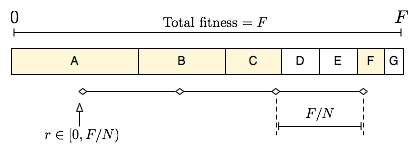
\includegraphics[scale=0.6]{images/sus.png}
\caption[Stochastic Universal Sampling (Pointer Intervals)]{Beginning at a random starting point on the interval $[0,fitness\_sum]$, stochastic universal sampling (SUS) uses evenly spaced pointers to select rules (Source: \cite{assumed_diagram_2007})}
\label{sus_graphic}
\end{figure}

Algorithm \ref{sus} shows SUS in pseudocode. It will help, in understanding the behavior of SUS, to imagine the interval $[0, fitness\_sum]$ on the real number line. Additionally, imagine that each member of the population is given its own subinterval within the $[0, fitness\_sum]$ that is equivalent in length to its fitness. (See figure \ref{sus_graphic}.)

To begin, a value known as the ``pointer interval'' is computed by dividing the sum of the fitnesses (\emph{fitness\_sum}) by the number of rules to be selected ($N$). Then, a random number $r$ is chosen from the range $[0, pointer\_interval]$. Beginning at $r$, the algorithm selects $N$ positions along $[0, fitness\_sum]$ by counting out intervals of length $pointer\_interval$. The rules corresponding to the subintervals in which the positions fall are the ones selected.

\subsubsection{Genetic Operators and Replacement}

At each iteration, a fixed number of the fittest rules from the previous generation are added to the next generation. This number is expressed as a fraction of the population size in the \emph{elitism\_rate} parameter, and the rules thus selected are said to be ``elite.'' The rest of the population for the next generation is filled via crossover and mutation of the rules chosen to reproduce during the selection phase.

\emph{Crossover}. The GA uses single-point crossover. For every set of parents, a random integer in the range $[1, num\_attributes - 1]$ is selected as the crossover point. The condition of each of the offspring rules is created by swapping the attribute values to the right of the crossover point in each of the parents. The values of the attributes' \emph{dont\_care} variables are also preserved.

\emph{Mutation}. After crossover, the mutation operator iterates over the condition attributes of each offspring. Each attribute has the same probability of being modified (\emph{p\_mutate}). If it has been determined that an attribute is to be mutated, a second random number in the interval $[0,1]$ is generated. If that number is less than or equal to a probability \emph{p\_dont\_care}, the attribute's \emph{dont\_care} variable is set to true. If the number is greater than \emph{p\_dont\_care}, the attribute is randomly assigned a new quantile.

After both operators have been applied, all of the offspring replace all of the non-elite ($pop\_size - N$) members of the current generation. The resulting population thus forms the next generation.

\subsection{Classification of Examples}

Classification of examples in the test set is straightforward. At the end of \textit{num\_gens} generations, the genetic algorithm terminates. Only the rules in the final population that (a) are elite and that (b) have more true positives than false positives are used for the classification task. There are several reasons for these criteria:
\begin{enumerate}
\item The elite rules in the final population are (mostly) those that have weathered repeated applications of the selection procedure and have proved themselves effective. Among the non-elites, which will have just been generated through crossover and mutation in the final generation, there are likely to be many bad rules.
\item We are interested in minimizing the number of rules needed to accurately characterize the target class.
\item Rules that incorrectly identify negative instances more frequently than they correctly identify positive ones would only diminish the accuracy of the system.
\end{enumerate}

The number of rules used for the classification may therefore never exceed $pop\_size * elitism\_rate$. Once these rules have been identified, the LCS iterates over the examples in the test set. If a rule that covers the current example is found among the set selected, the example is classified as a member of the target class. If no matching rule is found, the example is classified as a member of the default class.\footnote{Since the system attempts to characterize just one class per run (the target class), it does not matter what is chosen for the default class, so long as it is different from the target class.} After a class has been selected for the example, the system compares the selected class with the actual class of the example and categorizes it accordingly as a true positive, true negative, false positive, or false negative. The tallies of all four categories are outputted once all examples have been classified and relevant statistics are calculated.

\subsection{Parameters}

The system takes the following arguments:

\begin{description}
\item \textit{pop\_size:} the number of rules in the population.
\item \textit{num\_gens:} the number of generations the LCS will run before terminating.
\item \textit{target\_class:} the class in the training data that the LCS will attempt to characterize.
\item \textit{elitism\_rate:} the approximate fraction of the population that is to be retained from one generation to the next.
\item \textit{p\_mutate:} the probability that a condition attribute will be mutated when the mutation operator is invoked.
\item \textit{p\_dont\_care:} if it has been determined that an attribute is to be mutated, the probability that its \textit{dont\_care} variable will be set to true (instead of assigning it a new quantile).
\item \textit{training\_set:} an object containing all of the examples in the training set and other relevant information.
\item \textit{test\_set:} an object containing all of the examples in the test set and other relevant information.
\end{description}

\section{Experiment and Results}

\subsection{Preliminary Evaluation on Small Data Sets}

As a benchmark test, I evaluated the system's performance on the Iris and Wine data sets from the UC-Irvine Machine Learning Repository \cite{noauthor_uci_nodate-1,noauthor_uci_nodate}. Details of the data sets are shown in tables \ref{iris_info} and \ref{wine_info} in appendix A.\footnote{All tables mentioned hereafter can be found in the appendices.} For both sets, quartiles were computed for each non-class attribute based on the range of values for that attribute across all examples in the target class. The population was then initialized with \textit{pop\_size} rules whose attributes are assigned random quartile values. Trial runs revealed that parameter values of \textit{pop\_size} = 40, \textit{num\_gens} = 1000, \textit{elitism\_rate} = 0.6, \textit{p\_mutate} = 0.25, and \textit{p\_dont\_care} = 0.3 work well. Ten experiments were run per class on each set using a simple holdout method with training and test sets of approximately equal size. Tables \ref{iris_results} and \ref{wine_results} show the mean accuracy, odds ratio, true positives, true negatives, false positives, false negatives, and number of rules used for classification for Iris and Wine, respectively. 

The LCS performed fairly on these simpler sets, achieving a weighted mean accuracy of 94.1\% for the Iris test sets and 89.9\% for the Wine sets. In both cases, the number of rules used for classification was reasonably compact (about 5.1 per class on Iris and 8.4 per class on Wine). Although a discrepancy in performance is to be expected between training and testing sets in most supervised learning tasks, the accuracy difference between those sets in the case of the Wine data hinted at potential problems with overfitting. This would be somewhat surprising considering the selection pressure  for more general rules (via the fitness bonus for those rules with more ``don't care'' attributes). But to make any confident statements on this point required results from tests on the yield data.

\subsection{Experiments on Yield Data}

\subsubsection{Setup}
In their experiments, Nelson and Congdon looked at two data sets, one of which contained fertilizer as an attribute, and the other of which did not. Time constraints permitted me to examine just one of these , and I chose the latter, as it contains data for countries up through 2007, while the former stops at 2002. From this original set, Nelson and Congdon derived twelve (non-disjoint) subsets by adjusting the following variables:
\begin{enumerate}
\item \textit{Year.} Indicates whether or not the year is included as an attribute of the examples. The purpose of splitting the data in this way is to evaluate the effect that time exhibits on yield changes, independent of the other variables. This variable essentially comprises all other factors that influence yield but that are not considered as attributes of the data.
\item \textit{Region.} Indicates whether the data set includes data from countries in the tropics, countries in the temperate regions, or both (global). Looking at the data by region may reveal differences in which attributes have the most significant influence on yield.
\item \textit{Yield Units.} Indicates whether the change in yield is expressed as Mg/ha or Mkcal/ha. Framing the data in terms of both mass and energy simply offers different ways of understanding yield.
\end{enumerate}
Thus, two possibilities  each for the \textit{year} and \textit{yield units} variables, and three possibilities for the \textit{region} variable give twelve data sets. Since I was examining annual change in the various inputs, however, it made no sense to include the year attribute, and so I ran my experiments on the six data sets in which the year was omitted. The class attribute, change in yield, was discretized to tertiles (``high'' (H), ``medium'' (M), and ``low'' (L) change) as it was in Nelson and Congdon's work. The non-class attributes were discretized into quartiles, after some preliminary tests showed them to be preferable to tertiles, quintiles, and sextiles.\footnote{See table \ref{crop_attributes} for a listing of all attributes.}

I performed five ten-fold cross validations per data set per class. Good parameter values were determined through experimentation and consultation of the literature. Ultimately, I maintained the values of \textit{elitism\_rate} (0.6), \textit{p\_mutate} (0.25), and \textit{p\_dont\_care} (0.3) used on the Iris and Wine sets, but increased \textit{pop\_size} to 300 and \textit{num\_gens} to 2500.

\subsubsection{Performance}

Tables \ref{k.ny.temp_results} through \ref{t.ny.wt_results} show averages of the results of the five ten-fold cross validations. A quick survey of the data reveals at least two interesting patterns.

First, the system exhibits a reasonably high degree of accuracy on the training sets, particularly on the temperate and tropical data, where it achieved mean accuracies of 95.0\% and 96.0\%, respectively. Performance on the global data was noticeably worse (with a mean accuracy of about 87.2\%), but such a result is unsurprising, considering that the global sets included both temperate and tropical examples, which renders the task of generating accurate, yet general rules substantially more difficult. The strength of the system's performance on the training sets is perhaps most evident in its near-complete avoidance of false positives. This is no doubt partly a consequence of the restriction that all rules to be used in the classification task must have more true positive examples than false positives ones. But even with this criterion, one might still expect to see at least some false positive examples. I return this topic in section 5.

Second, performance declined substantially on the test sets. The mean accuracy was 65.4\% on the temperate data, 59.2\% on the tropical, and 66.6\% on the global. These observations, in conjunction with the relatively strong performance on the training set, seem to reinforce the conclusion that the system struggles with overfitting.

\subsubsection{Calculating Relative Impact}

To determine the relative impacts of the different factors on yield, I considered the number of true positives identified in each of the six data sets. First, for each rule $R$ used in the classification of a given set, I found all of the attributes not marked as ``don't cares.'' Suppose that rule $R$ has $N$ such attributes and covers $|TP|_R$ true positive examples. Then each of the $N$ attributes is awarded $\frac{|TP|_R}{N}$ points for its part in ``explaining'' the $|TP|_R$ true positive examples. By repeating this procedure for every rule used in the classification, tallying the number of points for each attribute in the data set, and finally dividing the tallies by the total number of true positives, I obtained percentages of the number of true positives explained by each of the attributes. Tables \ref{temperate_percentages} through \ref{global_percentages} present the results of this analysis. 

Next, I broke down the number of true positives explained by an attribute based on quartile. For a given attribute $A$ and class $c$, I found the fraction of $A$'s true positive examples of class $c$ that are explained by each quartile. This finer-grain perspective allows one to see \emph{how} the various attributes correlate with changes in overall yield. See tables \ref{k.ny.temp.quartiles} through \ref{t.ny.wt.quartiles}.

\subsubsection{Predictive Factors}

My results support several of the findings in \cite{nelson_measuring_2016}. For one, they reinforce Nelson and Congdon's conclusion that crop mix exerted a greater influence on the change in overall yield than any other factor, regardless of the magnitude of change. In all but two cases, crop mix accounted for more than 50\% of true positive examples. Furthermore, within the crop mix vector, sugarcane covered the greatest number of examples in the temperate and global data sets, and increases in sugarcane production appear to be strongly positively correlated with overall gains in yield. In temperate regions, an average of 51\% of the examples from the high class that are explained by the sugarcane attribute are associated with the top quartile, while only 9.1\% fall in the bottom quartile. By contrast, of examples in the low class, an average of 49.2\% belong to the bottom quartile, and just 5\% to the top quartile. The authors' decision tree analysis bore similar results. Apart from sugarcane, however, the crops show a remarkable degree of uniformity in their relative impacts, and most noticeably in the tropics. In both tropical data sets, no single attribute accounted for less than 3.7\% (total cropped hectarage) or more than 8.9\% (roots and tubers) of the true positive examples, and percentages for the other attributes exhibit a fairly even distribution within that range. 

Additionally, the results corroborate the authors' finding that investment in land and machinery represents a lesser fraction of examples when compared with crop mix and climate. Collectively, these two variables were responsible for an average of about 11.8\% of true positives, while crop mix and climate covered averages of about 53.7\% and 16.9\%, respectively. In temperate regions, particularly when yield was measured in Mkcal/ha, there was a strong positive correlation between machinery investments and overall yield change: of true positives from the high class that were explained by the ``eqp'' attribute, 51.2\% were associated with the top quartile, and 40.6\% of those in the low class were associated with the bottom quartile. In the medium class, a combined 71\% of examples fell in the middle two quartiles. Curiously, no such relationship obtained in either the tropical or global data.

Soil quality and cropped footprint had still less of an effect than land and machinery investment and explained an average of roughly 4.7\% and 5.2\% percent of examples. Irrigation was found to have a similarly minimal impact, with an average of under 5.6\%. The data also failed to reveal any clear relationship between changes in any of the three variables and yield gains. Both the decision tree and regression analyses in \cite{nelson_measuring_2016} support the same conclusions.

For all of these parallels, however, there is at least one important point of divergence between the findings in \cite{nelson_measuring_2016} and my own. Nelson and Congdon note that changes in climate (which includes the daytime and nighttime growing season temperature and growing season precipitation variables) had only a ``slight'' effect on yields. Particularly surprising is their judgment that precipitation had virtually no influence at all. In my analysis, by contrast, the climate attributes explained nearly 17\% of positive examples, which can hardly be considered a negligible impact.\footnote{It should be noted that in the decision tree analysis in \cite{nelson_measuring_2016}, the daytime growing season temperature was found close to the root in tropical countries, which suggests a significant impact.} Moreover, across all regions, a rise in average daytime growing season temperature correlated with yield losses. Nighttime temperatures exhibited a similar trend, though less pronounced. These relationships may hint at the damaging influence of global warming on agricultural output.

\subsubsection{Discussion}

Nelson and Congdon conclude the introduction of their paper with the following prescription for maintaining global yield levels:

\begin{displayquote}
Our results indicate that 1) transferring technology and other inputs to the tropics 2) encouraging countries to exclusively concentrate on growing the crops most suited to their soil-climate conditions (and trading for the rest of the crops their consumers want), and 3) increasing the productivity of existing cropland in lieu of additional cropland extensification will be the most effective ways to ameliorate climate change's expected drag on global yields \cite{nelson_measuring_2016}.
\end{displayquote}

In the introduction to this paper, I asserted that my project attempts merely to evince correlations between agricultural inputs and changes in yield, and that one ought not infer policy recommendations from those correlations. With all due respect to Nelson and Congdon's work, and regardless of the prudence of the measures they advise here, I do not believe that the data underlying both their analysis and mine are sufficiently numerous or comprehensive to merit any meaningful prognosis about what will or will not prove effective agricultural praxis in the face of climate change. Understanding the interaction of the variables examined here is a task of exceptional complexity, and solutions to global problems must be crafted with great care. At most, these investigations should be a guide for future inquiry into the relationships between economic and environmental factors on the one hand, and agricultural output on the other.

\section{Future Work and Conclusion}

In this paper, I presented a Michigan-style, real-valued LCS designed to establish a relationship between the change in various country-level agricultural inputs and the change in overall agricultural yield. Specifically, I investigated data collected by Erik Nelson, previously analyzed in a 2016 paper by Nelson and Congdon. In section 2, I offered some background on the GBML paradigm, on LCSs in general, and on several milestones in the research on LCSs for supervised learning. In section 3, I outlined the design of my own LCS, and in section 4 I reported on the performance of the LCS both on sample data sets from the UCI Machine Learning Repository and on Nelson's agricultural data. In the remainder of this final section, I discuss directions for future work.

\subsection{Accuracy}
The results of this project reveal many potential avenues for improvement and further experimentation. Plainly, the performance of the system on the ten-fold cross validations indicates that changes must be made to improve accuracy. Several possibilities suggest themselves. 

For one, the system could conceivably be enhanced by using a different fitness function. Although the log of the odds ratio makes intuitive sense, performance can nonetheless be hindered when the best rules in the population have fitnesses that exceed those of the less effective rules, as the top few rules will tend to dominate and cause the population to converge prematurely. Rank-based fitness, in which individuals are assigned a fixed fitness value based on their rank in the population, could provide a solution. Initial tests using a naive rank-based fitness algorithm produced mixed results, but more sophisticated algorithms could yield significant gains in accuracy.

The system may further benefit from additional genetic operators. An operator like Pier Lanzi's \emph{specify}, which periodically generates rules directly from examples, could help to counteract premature convergence and to encourage greater coverage of the training set \cite{lanzi_study_1997}.

Lastly, an alternative attribute representation could also contribute to greater accuracy. Given that the attributes of Nelson's data are all continuous-valued, a fuzzy representation such as the one proposed in 
Valenzuela-Rend\'on's FCS could allow for more flexible rules, as well as a more descriptive characterization of the change in yield \cite{manuel_valenzuela-rendon_fuzzy_1991}.

In 4.2.2, I noted that the system appears to struggle with overfitting, and it is not clear to what extent these possible changes would remedy the problem. I also highlighted the small number of false positives that were observed on the training sets, and suggested that this is likely in part due to the criterion that no rule to be used in the classification may have more true positive examples than false positive ones. Yet, it seems to have more to do with the lack of any criterion for the minimum \emph{number} of true positives a rule must have. The problem of not having such a restriction is that rules could be generated that cover just a few true positive examples, but that nonetheless achieve a sufficiently high fitness to be considered ``elite'' and so survive unchanged until the end of a run. Those rules will then be selected for use in the classification task, but will likely be overly specific and thus fail to correctly identify positive examples in the test set. If there are too many of these over-specific rules, performance will suffer.

Upon examination of some of the final rule sets, I did find a high proportion of rules that covered only several examples. Given that the system already has a reward mechanism for more general rules, it is puzzling why this problem would persist. Resolving it would be a top priority for future research.

\subsection{Data}

In addition to accuracy improvements, the project would also benefit from more and different kinds of data. This paper concerns itself with just one of the two original data sets that Nelson and Congdon investigated --- namely, the one in which fertilizer data is absent. Considering the disagreement between the regression and decision tree analyses on the importance of fertilizer, it would valuable to have a third opinion. Moreover, to obtain a more comprehensive picture of the environmental and economic influences on yields, fertilizer use, as well as other variables like GDP, population, and the presence of plant disease, must be considered. So long as we are interested in year-to-year changes in yield (and not absolute quantities), neither decision trees nor LCSs can account for other, ``unobserved'' factors in the way that fixed effects modeling permits. Absent that ability, the best means of improving our understanding through those models is to take more variables into account.


\titleformat{\section}{\large\bfseries}{\appendixname~\thesection .}{0.5em}{}
\titleformat{\subsection}{\normalsize\bfseries}{\thesubsection .}{0.5em}{}
\appendix
\appendixpage
\addappheadtotoc

\section{Results for Iris and Wine Data Sets}

The results shown in tables \ref{iris_results} and \ref{wine_info} reflect averages across ten holdout experiments for each class. All entries in the tables apart from the ``Type'' and  ''Class'' are averages across ten tests. ``Type'' denotes the kind of set (testing or training); ``Class'' refers to the target class; ``Size'' is the average number of examples in the target class; ``Acc'' is the overall accuracy; ``lnOR'' is the average of the natural log of the odds ratio; ``TP,'' ``TN,'' ``FP,'' and ``FN,'' are the average numbers of true positives, true negatives, false positives, and false negatives; and ``\# Rules'' indicates the average number of rules actually used to classify the examples.

% iris info
\begin{table}[h!]
\centering
\begin{tabular}{ll}
\toprule
\multicolumn{2}{c}{\textbf{Iris}} \\
\midrule
Number of Examples: & 150 \\
Classes: & Iris-Setosa (50), Iris-Versicolour (50), \\
& Iris-Virginica (50) \\
Number of Non-Class Attributes: & 4 \\
Non-Class Attribute Value Types: & Real \\
Non-Class Attributes: & sepal length, sepal width, \\
& petal length, petal width \\
\bottomrule
\end{tabular}
\caption[Iris Data Set Information]{The Iris dataset from the UCI Machine Learning Repository.}
\label{iris_info}
\end{table}

% iris results
\begin{table}[h!]
\centering
\begin{tabular}{llllllllll}
\toprule
\multicolumn{10}{c}{\textbf{Iris}}  \\
\midrule
Type & Class & Size & Acc & lnOR & TP & TN & FP & FN & \# Rules \\
\midrule
Training & Setosa & 25.0 & 1 & 8.553 & 25.0 & 50.4 & 0 & 0 & 4.2 \\
& Versicolour & 25.2 & 0.981 & 7.218 & 24 & 50 & 0.2 & 1.2 & 5.9 \\
& Virginica & 25.2 & 0.981 & 7.558 & 24 & 50.2 & 0 & 1.2 & 5.3 \\
Testing & Setosa & 25.0 & 0.983 & 7.570 & 24.5 & 48.8 & 0.8 & 0.5 & 4.2 \\
& Versicolour & 24.8 & 0.89 & 4.120 & 19.8 & 26.6 & 3.2 & 5.0 & 5.9 \\
& Virginica & 24.8 & 0.95 & 5.664 & 22.1 & 48.8 & 1 & 2.7 & 5.3 \\
\bottomrule
\end{tabular}
\caption[Results for the Iris Data Set]{Averages of 10 holdout tests for each class in the Iris data set.}
\label{iris_results}
\end{table}

% wine info
\begin{table}[h!]
\centering
\begin{tabular}{ll}
\toprule
\multicolumn{2}{c}{\textbf{Wine}} \\
\midrule
Number of Examples: & 178 \\
Classes: & class 1 (59), class 2 (71), class 3 (48) \\
Number of Non-Class Attributes: & 13 \\
Non-Class Attribute Value Types: & Integer, Real \\
Non-Class Attributes: & Alcohol, Malic Acid, Ash \\ & Alcalinity of Ash, Magnesium, \\
& Total phenols, Flavanoids, \\
& Nonflavanoid phenols, \\
& Proanthocyanins, \\
& Color intensity, Hue, \\
& OD280/OD315 of diluted wines, \\
& Proline \\
\bottomrule
\end{tabular}
\captionsetup{width=.9\textwidth}
\caption[Wine Data Set Information]{The Wine dataset from the UCI Machine Learning Repository. The names for the class attribute values are not specified.}
\label{wine_info}
\end{table}

% wine results
\begin{table}[h!]
\centering
\begin{tabular}{llllllllll}
\toprule
\multicolumn{10}{c}{\textbf{Wine}} \\
\midrule
Type & Class & Size & Acc & lnOR & TP & TN & FP & FN & \# Rules \\
\midrule
Training & 1 & 30.3 & 1 & 8.895 & 30.3 & 58.8 & 0 & 0 & 9.7 \\
& 2 & 35.0 & 1 & 8.955 & 35.0 & 54.1 & 0 & 0 & 8.7 \\
& 3 & 23.8 & 1 & 8.763 & 23.8 & 65.3 & 0 & 0 & 6.4 \\
Testing & 1 & 29.7 & 0.841 & 3.333 & 24.8 & 50.0 & 9.2 & 4.9 & 9.7 \\
& 2 & 35.0 & 0.919 & 4.894 & 30.4 & 51.3 & 2.6 & 4.6 & 8.7 \\
& 3 & 24.2 & 0.939 & 5.626 & 20.7 & 62.8 & 1.9 & 3.5 & 6.4 \\
\bottomrule
\end{tabular}
\caption[Results for the Wine Dataset]{Averages of 10 holdout tests for each class in the Wine data set.}
\label{wine_results}
\end{table}
\clearpage

\section{Results for Crop Yield Data}
\subsection{Attributes}
Table \ref{crop_attributes} shows the attributes of the yield data. All but three of the attributes (``tropical,'' ``Mkcal/ha,'' ``Mg/ha'') are present in all of the data sets. Recall that half of the data sets express change in yield in Mkcal/ha, while the other half express it in Mg/ha. The ``tropical'' attribute is to be found only in the global data, since it would contribute nothing in the temperate and tropical data sets. Except for ``tropical,'' each of the attributes in the table should be interpreted as the annual \emph{change} in the metric described --- not as an absolute quantity. 

\begin{table}[h!]
\centering
\begin{tabular}{ll}
\toprule
\textbf{Attribute} & \textbf{Description} \\
\midrule
tropical* & An indicator denoting whether the country is tropical \\
& or temperate. \\
soil & The composite soil quality score (on a 1 to 5 scale, with lower \\
& numbers indicating better soil). \\
ha & Total cropped hectares. \\
rice & Cropped rice as a percentage of total cropped area. \\
wheat & Cropped wheat as a percentage of total cropped area.\\
sugar & Cropped sugar as a percentage of total cropped area.\\
grains & Cropped coarse grains as a percentage of total cropped area.\\
oil & Cropped oil crops as a percentage of total cropped area.\\
fruits & Cropped fruits as a percentage of total cropped area.\\
roots & Cropped roots and tubers as a percentage of total cropped area.\\
other & All other cropped produce as a percentage of total cropped area. \\
davg & Average daytime growing season temperature. \\
navg & Average nighttime growing season temperature. \\
pavg & Total rainfall (in mm) over cropped lands during \\
& the growing season. \\
irr & Fraction of cropped lands equipped for irrigation. \\
land & Total money (in 2005 USD) invested in agricultural \\
& land development divided by cropped hectares. \\
eqp & Total money (in 2005 USD) invested in agricultural \\
&  equipment divided by cropped hectares. \\
Mkcal/ha* & Total crop yield in metric tons per hectare. \\
Mg/ha* & Total crop yield in millions of kilocalories per hectare. \\
\bottomrule 
\end{tabular}
\captionsetup{width=.95\textwidth}
\caption[Attribute Descriptions for Yield Data]{Attributes of the crop yield data. Attribute names followed by a ``*'' indicate that the attribute is not used in all data sets. Descriptions were taken with some modification from \cite{nelson_measuring_2016}.}
\label{crop_attributes}
\end{table}

\subsection{Performance}
The results for each class in tables \ref{k.ny.temp_results} through \ref{t.ny.wt_results} reflect averages across five ten-fold cross validations. Tables \ref{k.ny.temp_results} and \ref{t.ny.temp_results} show results for temperate countries, tables \ref{k.ny.trop_results} and \ref{t.ny.trop_results} for tropical countries, and \ref{k.ny.wt_results} and \ref{t.ny.wt_results} for all countries. In all experiments, the LCS used the maximum number of rules allowed given the parameters (180). Consequently, the ``\# Rules'' column has been omitted. The number of examples in each set is shown in parentheses in the ``Type'' column.
\\
\\
\\
% 1. temperate, Mkcal/ha
\begin{table}[h!]
\centering
\begin{tabular}{lllllllll}
\toprule
\multicolumn{9}{c}{\textbf{Temperate, Mkcal/ha}} \\
\midrule
Type & Class & Size & Acc & lnOR & TP & TN & FP & FN \\
\midrule
Training & H & 591.3 & 0.956 & 9.68 & 510.0 & 1280.7 & 0 & 81.3  \\
(1872) & M & 675.0 & 0.938 & 9.35 & 558.5 & 1197.0 & 0 & 116.5  \\
& L & 603.4 & 0.953 & 9.61 & 915.6 & 1268.6 & 0 & 87.8  \\
Testing & H & 59.1 & 0.650 & 1.32 & 32.8 & 102.3 & 28.6 & 27.6  \\
(208) & M & 75.0 & 0.658 & 1.08 & 35.98 & 101.2 & 31.8 & 40.0  \\
& L & 69.6 & 0.664 & 1.06 & 34.6 & 103.6 & 34.8 & 35.1  \\
\bottomrule
\end{tabular}
\captionsetup{width=.85\textwidth}
\caption[Performance on Temperate Data with Yield in Mkcal/ha]{Performance on examples from countries in temperate regions with yield measured in Mkcal/ha.}
\label{k.ny.temp_results}
\end{table}

% 2. temperate, Mg/ha
\begin{table}[h!]
\centering
\begin{tabular}{lllllllll}
\toprule
\multicolumn{9}{c}{\textbf{Temperate, Mg/ha}} \\
\midrule
Type & Class & Size & Acc & lnOR & TP & TN & FP & FN \\
\midrule
Training & H & 529.2 & 0.965 & 9.85 & 463.8 & 1342.8 & 0 & 65.38  \\
(1872) & M & 746.1 & 0.935 & 9.36 & 625.1 & 1125.9 & 0 & 121.0  \\
& L & 596.0 & 0.951 & 9.55 & 504.2 & 1276.0 & 0 & 91.8  \\
Testing & H & 53.5 & 0.636 & 1.24 & 28.36 & 103.9 & 28.8 & 25.1  \\
(208) & M & 82.9 & 0.634 & 0.97 & 41.9 & 89.8 & 35.3 & 41.0  \\
& L & 67.0 & 0.679 & 1.20 & 34.6 & 106.5 & 34.5 & 32.4  \\
\bottomrule
\end{tabular}
\captionsetup{width=.85\textwidth}
\caption[Performance on Temperate Data with Yield in Mg/ha]{Performance on examples from countries in temperate regions with yield measured in Mg/ha.}
\label{t.ny.temp_results}
\end{table}

\clearpage
% 3. tropics, Mkcal/ha
\begin{table}[h!]
\centering
\begin{tabular}{lllllllll}
\toprule
\multicolumn{9}{c}{\textbf{Tropical, Mkcal/ha}} \\
\midrule
Type & Class & Size & Acc & lnOR & TP & TN & FP & FN \\
\midrule
Training & H & 589.5 & 0.95 & 9.562 & 511.8 & 1080.9 & 0 & 77.7  \\
(1670) & M & 505.8 & 0.964 & 9.76 & 445.9 & 1164.6 & 0 & 59.9  \\
& L & 575.6 & 0.958 & 9.66 & 505.29 & 1094.8 & 0 & 70.3  \\
Testing & H & 65.5 & 0.569 & 0.256 & 25.8 & 79.9 & 40.2 & 39.7  \\
(186) & M & 56.2 & 0.595 & 0.317 & 21.7 & 88.8 & 040.6 & 34.5  \\
& L & 63.4 & 0.590 & 0.449 & 27.4 & 82.1 & 40.1 & 36.0  \\
\bottomrule
\end{tabular}
\captionsetup{width=.85\textwidth}
\caption[Performance on Tropical Data with Yield in Mkcal/ha]{Performance on examples from countries in tropical regions with yield measured in Mkcal/ha.}
\label{k.ny.trop_results}
\end{table}

% 4. tropics, Mg/ha
\begin{table}[h!]
\centering
\begin{tabular}{lllllllll}
\toprule
\multicolumn{9}{c}{\textbf{Tropical, Mg/ha}} \\
\midrule
Type & Class & Size & Acc & lnOR & TP & TN & FP & FN \\
\midrule
Training & H & 651.6 & 0.952 & 9.58 & 571.4 & 1018.8 & 0 & 80.2  \\
(1670) & M & 434.7 & 0.973 & 9.94 & 390.2 & 1235.7 & 0 & 44.5  \\
& L & 584.4 & 0.96 & 9.71 & 516.7 & 1086.1 & 0 & 67.7  \\
Testing & H & 72.4 & 0.572 & 0.415 & 31.7 & 74.5 & 38.7 & 40.7  \\
(186) & M & 48.3 & 0.639 & 0.517 & 18.4 & 100.3 & 37.0 & 29.9  \\
& L & 64.6 & 0.587 & 0.429 & 27.9 & 81.0 & 39.9 & 36.7  \\
\bottomrule
\end{tabular}
\captionsetup{width=.85\textwidth}
\caption[Performance on Tropical Data with Yield in Mg/ha]{Performance on examples from countries in tropical regions with yield measured in Mg/ha.}
\label{t.ny.trop_results}
\end{table}

% 5. global Mkcal/ha
\begin{table}[h!]
\centering
\begin{tabular}{lllllllll}
\toprule
\multicolumn{9}{c}{\textbf{Global, Mkcal/ha}} \\
\midrule
Type & Class & Size & Acc & lnOR & TP & TN & FP & FN \\
\midrule
Training & H & 1180.8 & 0.874 & 9.00 & 733.6 & 2361.6 & 0 & 447.2  \\
(3542) & M & 1180.8 & 0.866 & 8.829 & 704.4 & 2361.6 & 0 & 476.4  \\
& L & 1178.6 & 0.871 & 8.86 & 723.2 & 2363.7 & 0.1 & 455.4  \\
Testing & H & 131.2 & 0.667 & 0.93 & 44.1 & 218.4 & 44.0 & 87.1  \\
(394) & M & 131.2 & 0.659 & 0.80 & 40.0 & 219.5 & 42.9 & 91.4  \\
& L & 133.4 & 0.662 & 0.90 & 42.6 & 218.0 & 42.2 & 90.8  \\
\bottomrule
\end{tabular}
\captionsetup{width=.85\textwidth}
\caption[Performance on Global Data with yield in Mkcal/ha]{Performance on examples from all countries with yield expressed in Mkcal/ha.}
\label{k.ny.wt_results}
\end{table}
\clearpage

% 6. temperate and tropics, Mg/ha
\begin{table}[h!]
\centering
\begin{tabular}{lllllllll}
\toprule
\multicolumn{9}{c}{\textbf{Global, Mg/ha}} \\
\midrule
Type & Class & Size & Acc & lnOR & TP & TN & FP & FN \\
\midrule
Training & H & 1180.8 & 0.880 & 9.01 & 754.5 & 2361.6 & 0 & 426.3  \\
(3542) & M & 1180.8 & 0.872 & 8.93 & 727.2 & 2361.6 & 0 & 453.6  \\
& L & 1182.1 & 0.871 & 8.92 & 724.9 & 2360.4 & 0 & 457.2  \\
Testing & H & 131.2 & 0.672 & 0.99 & 45.3 & 219.2 & 43.4 & 85.9 \\
(394) & M & 131.2 & 0.660 & 0.84 & 42.6 & 217.3 & 45.1 & 88.6 \\
& L & 129.9 & 0.674 & 0.98 & 43.4 & 221.7 & 41.9 & 86.5 \\
\bottomrule
\end{tabular}
\captionsetup{width=.85\textwidth}
\caption[Performance on Global Data with Yield in Mg/ha]{Performance on examples from all countries and with yield expressed in Mg/ha.}
\label{t.ny.wt_results}
\end{table}

%%%%%%%%%%%%%%% ATTRIBUTE PERCENTAGES %%%%%%%%%%%%%%%%
\subsection{Impacts of Different Inputs}
Tables \ref{temperate_percentages} through \ref{global_percentages} indicate the relative importance of the different attributes in classifying examples from the six data sets. The values in the tables are average percentages of the total true positives identified in the training set that are explained by each attribute. Section 4.2.3 gives a more detailed account of how these percentages were calculated. Observe the additional attributes ``crop mix,'' ``climate,'' and ``land/eqp.'' These are aggregates of the atomic attributes shown in table \ref{crop_attributes} that Nelson and Congdon used in their analysis, and which I have included for ease of comparison. ``Crop mix'' combines ``rice,'' ``wheat,'' ``sugar,'' ``grains,'' ``oil,'' ``fruits,'' ``roots,'' and ``other''; ``climate'' combines ``davg,'' ``navg,'' and ``pavg''; and ``land/eqp'' combines ``land'' and ``eqp.'' 

Tables \ref{temperate_percentages} through \ref{t.ny.wt.quartiles} break down the true positives explained by each attribute into quartiles. Specifically, for each non-class attribute $A$ and class $c$, they show the percentage of $A$'s true positives of class $c$ that are explained by each quartile. This information provides a sense of the \emph{kind} of correlation between the change in $A$ and the change in yield. All tables concerning relative impacts (\ref{k.ny.temp.quartiles} through \ref{t.ny.wt.quartiles}) reflect averages from a single ten-fold cross validation.

% 7. temperate, Mkcal/ha
\begin{table}
\centering
\parbox{.45\linewidth} {
\begin{tabular}{llll}
\toprule
\multicolumn{4}{c}{\textbf{Temperate, Mkcal/ha}} \\
\midrule
Attribute & High & Medium & Low \\
\midrule
soil & 4.7 & 4.6 & 5.5 \\
ha & 6.2 & 5.8 & 4.8 \\
rice & 6.3 & 6.6 & 4.8 \\
wheat & 5.4 & 5.5 & 6.6 \\
sugar & 16.7 & 13.2 & 16.8 \\
grains & 6.1 & 5.4 & 6.6 \\
oil & 4.4 & 4.9 & 5.4 \\
fruits & 6.3 & 5.7 & 4.1 \\
roots & 6.9 & 4.5 & 5.1 \\
other & 4.6 & 6.6 & 6.3 \\
davg & 6.0 & 4.5 & 6.3 \\
navg & 4.1 & 5.2 & 5.0 \\
pavg & 6.2 & 5.2 & 5.7 \\
irr & 4.2 & 8.4 & 4.6 \\
land & 4.8 & 5.4 & 7.0 \\
eqp & 7.0  & 8.4 & 5.0 \\
\midrule
crop mix & 56.7 & 52.4 & 55.7 \\
climate & 16.3 & 14.9 & 17.0 \\
land/eqp & 11.8 & 13.8 & 12.0 \\
\bottomrule
\end{tabular}
\label{k.ny.temp_percentages}
}
% 8. temperate, Mg/ha
\parbox{.45\linewidth} {
\centering
\begin{tabular}{llll}
\toprule
\multicolumn{4}{c}{\textbf{Temperate, Mg/ha}} \\
\midrule
Attribute & High & Medium & Low \\
\midrule
soil & 4.4 & 4.0 & 4.1 \\
ha & 5.9 & 5.8 & 4.4 \\
rice & 6.2 & 5.2 & 5.2 \\
wheat & 4.8 & 7.4 & 6.9 \\
sugar & 14.2 & 10.7 & 14.0 \\
grains & 5.5 & 5.8 & 5.3 \\
oil & 4.6 & 5.1 & 6.6 \\
fruits & 7.9 & 7.1 & 5.9 \\
roots & 6.8 & 7.8 & 7.8 \\
other & 6.1 & 5.7 & 6.7 \\
davg & 6.1 & 4.8 & 6.0 \\
navg & 5.0 & 4.9 & 4.6 \\
pavg & 5.6 & 4.9 & 4.6 \\
irr & 6.1 & 6.7 & 5.7 \\
land & 4.5 & 6.4 & 7.2 \\
eqp & 6.2 & 7.8 & 4.9 \\
\midrule
crop mix & 56.1 & 54.8 & 59.4 \\
climate & 16.7 & 14.6 & 15.2 \\
land/eqp & 10.7 & 14.2 & 12.1 \\
\bottomrule
\end{tabular}
\label{t.ny.temp_percentages}
}
\captionsetup{width=.9\textwidth}
\caption[Percentage of Examples Explained by Attribute (Temperate Data)]{The average percentage of true positive examples explained by each attribute for temperate data. Values were computed from runs on temperate training sets (for yield in both Mkcal/ha and Mg/ha) from a single ten-fold cross validation.}
\label{temperate_percentages}
\end{table}

% 9. tropics, Mkcal/ha
\begin{table}[h!]
\centering
\parbox{.45\linewidth} {
\begin{tabular}{llll}
\toprule
\multicolumn{4}{c}{\textbf{Tropical, Mkcal/ha}} \\
\midrule
Attribute & High & Medium & Low \\
\midrule
soil & 5.4 & 5.3 & 4.9 \\
ha & 5.7 & 4.9 & 6.1 \\
rice & 6.1 & 6.1 & 5.3 \\
wheat & 7.9 & 6.3 & 6.3 \\
sugar & 5.6 & 3.9 & 6.5 \\
grains & 6.4 & 7.8 & 6.4 \\
oil & 8.9 & 5.8 & 8.0 \\
fruits & 5.9 & 7.4 & 6.5 \\
roots & 6.9 & 8.9 & 6.8 \\
other & 6.3 & 5.8 & 7.0 \\
davg & 6.8 & 7.2 & 6.6 \\
navg & 5.7 & 5.7 & 5.8 \\
pavg & 6.6 & 5.4 & 8.1 \\
irr & 5.2 & 5.4 & 4.2 \\
land & 4.8 & 5.7 & 5.6 \\
eqp & 5.8 & 8.3 & 6.0 \\
\midrule
crop mix & 54.0 & 52.0 & 52.8 \\
climate & 19.1 & 18.3 & 20.5 \\
land/eqp & 10.6 & 14.0 & 11.6 \\
\bottomrule
\end{tabular}
\label{k.ny.trop_percentages}
}
% 10. tropics, Mg/ha
\parbox{.45\linewidth} {
\centering
\begin{tabular}{llll}
\toprule
\multicolumn{4}{c}{\textbf{Tropical, Mg/ha}} \\
\midrule
Attribute & High & Medium & Low \\
\midrule
soil & 6.6 & 4.5 & 4.4 \\
ha & 4.1 & 3.7 & 6.2 \\
rice & 5.9 & 5.8 & 7.0 \\
wheat & 7.3 & 7.3 & 6.2 \\
sugar & 5.8 & 3.9 & 6.1 \\
grains & 4.4 & 8.0 & 6.8 \\
oil & 7.6 & 7.1 & 6.5 \\
fruits & 5.8 & 7.4 & 6.8 \\
roots & 7.0 & 6.7 & 7.5 \\
other & 8.8 & 6.4 & 8.3 \\
davg & 6.0 & 7.3 & 7.0 \\
navg & 7.6 & 6.8 & 5.9 \\
pavg & 7.1 & 6.4 & 6.3 \\
irr & 5.1 & 5.2 & 5.1 \\
land & 5.1 & 5.0 & 4.8 \\
eqp & 5.8 & 8.4 & 5.0 \\
\midrule
crop mix & 52.6 & 52.6 & 55.2 \\
climate & 20.7 & 20.5 & 19.2 \\
land/eqp & 10.9 & 13.4 & 9.8 \\
\bottomrule
\end{tabular}
\label{t.ny.trop_percentages}
}
\captionsetup{width=.9\textwidth}
\caption[Percentage of Examples Explained by Attribute (Tropical Data)]{The average percentage of true positive examples explained by each attribute for tropical data. Values were computed from runs on tropical training sets (for yield in both Mkcal/ha and Mg/ha) from a single ten-fold cross validation.}
\label{tropical_percentages}
\end{table}


% 11. global, Mkcal/ha
\begin{table}[h!]
\centering
\parbox{.45\linewidth} {
\begin{tabular}{llll}
\toprule
\multicolumn{4}{c}{\textbf{Global, Mkcal/ha}} \\
\midrule
Attribute & High & Medium & Low \\
\midrule
tropical & 5.1 & 8.6 & 5.2 \\
soil & 5.1 & 4.4 & 4.5 \\
ha & 4.5 & 5.6 & 5.0 \\
rice & 5.9 & 5.0 & 4.1 \\
wheat & 4.4 & 4.1 & 5.3 \\
sugar & 13.0 & 9.1 & 13.6 \\
grains & 6.8 & 6.8 & 7.2 \\
oil & 5.7 & 4.8 & 6.7 \\
fruits & 6.8 & 6.3 & 4.7 \\
roots & 7.3 & 5.8 & 5.5 \\
other & 5.7 & 5.1 & 5.8 \\
davg & 4.5 & 4.5 & 6.0 \\
navg & 4.7 & 3.9 & 6.2 \\
pavg & 4.6 & 5.4 & 4.7 \\
irr & 5.5 & 7.0 & 4.6 \\
land & 5.1 & 4.6 & 5.0 \\
eqp & 5.2 & 8.8 & 5.9 \\
\midrule
crop mix & 55.6 & 47.0 & 52.9 \\
climate & 13.8 & 13.8 & 16.9 \\
land/eqp & 10.3 & 13.4 & 10.9 \\
\bottomrule
\end{tabular}
\label{k.ny.wt_percentages}
}
% 24. global, Mg/ha
\parbox{.45\linewidth} {
\centering
\begin{tabular}{llll}
\toprule
\multicolumn{4}{c}{\textbf{Global, Mg/ha}} \\
\midrule
Attribute & High & Medium & Low \\
\midrule
tropical & 6.1 & 8.6 & 5.5 \\
soil & 4.7 & 3.9 & 4.4 \\
ha & 4.3 & 5.5 & 4.9 \\
rice & 5.8 & 5.9 & 5.0 \\
wheat & 4.1 & 5.7 & 5.8 \\
sugar & 12.3 & 7.6 & 12.0 \\
grains & 5.4 & 5.6 & 7.1 \\
oil & 6.1 & 5.6 & 7.6 \\
fruits & 5.9 & 7.8 & 7.9 \\
roots & 7.7 & 5.0 & 6.1 \\
other & 5.2 & 4.2 & 4.5 \\
davg & 4.6 & 4.4 & 6.3 \\
navg & 6.2 & 4.7 & 4.9 \\
pavg & 6.1 & 5.2 & 4.5 \\
irr & 5.1 & 6.9 & 4.9 \\
land & 4.4 & 4.2 & 4.9 \\
eqp & 5.8 & 9.2 & 3.8 \\
\midrule
crop mix & 52.5 & 47.4 & 56.0 \\
climate & 16.9 & 14.3 & 15.7 \\
land/eqp & 10.2 & 13.4 & 8.7 \\
\bottomrule
\end{tabular}
\label{t.ny.wt_percentages}
}
\captionsetup{width=.9\textwidth}
\caption[Percentage of Examples Explained by Attribute (Global Data)]{The average percentage of true positive examples explained by each attribute for tropical data. Values were computed from runs on tropical training sets (for yield in both Mkcal/ha and Mg/ha) from a single ten-fold cross validation.}
\label{global_percentages}
\end{table}

% 16. temperate, Mkcal/ha
\begin{sidewaystable}
\centering
\begin{tabular}{lllllllllllll}
\toprule
\multicolumn{13}{c}{\textbf{Temperate, Mkcal/ha}} \\
\midrule
& \multicolumn{4}{c}{High} & \multicolumn{4}{c}{Medium} & \multicolumn{4}{c}{Low} \\
\cmidrule(lr){2-5}
\cmidrule(lr){6-9}
\cmidrule(l){10-13}
Attribute & 1 & 2 & 3 & 4 & 1 & 2 & 3 & 4 & 1 & 2 & 3 & 4 \\
\midrule
soil & 17.3 & 31.2 & 22.0 & 29.5 & 26.6 & 30.8 & 24.8 & 17.8 & 24.0 & 19.9 & 25.9 & 30.2 \\
ha & 37.7 & 21.6 & 17.1 & 23.6 & 24.5 & 24.7 & 20.2 & 30.6 & 14.1 & 24.5 & 31.3 & 30.1 \\
rice & 37.7 & 16.3 & 24.9 & 21.2 & 14.3 & 35.2 & 34.3 & 16.2 & 31.8 & 25.4 & 15.1 & 27.8 \\
wheat & 27.9 & 20.8 & 20.3 & 30.9 & 22.0 & 24.5 & 19.0 & 34.4 & 31.2 & 20.2 & 22.7 & 25.8 \\
sugar & 8.8 & 4.5 & 37.2 & 49.6 & 6.0 & 30.1 & 49.2 & 14.7 & 42.9 & 33.3 & 20.7 & 3.2 \\
grains & 30.0 & 30.6 & 30.4 & 9.0 & 19.7 & 24.4 & 37.9 & 18.1 & 16.4 & 27.3 & 18.7 & 37.5 \\
oil & 24.1 & 19.3 & 21.5 & 35.2 & 17.6 & 34.8 & 29.4 & 18.1 & 41.6 & 26.4 & 17.1 & 14.9 \\
fruits & 20.0 & 18.6 & 44.0 & 17.4 & 20.4 & 32.2 & 36.4 & 11.1 & 37.0 & 23.5 & 15.1 & 24.4 \\
roots & 18.2 & 21.2 & 23.3 & 37.3 & 15.5 & 28.1 & 28.3 & 28.1 & 42.6 & 18.5 & 21.4 & 17.5 \\
other & 20.5 & 33.9 & 20.9 & 24.7 & 28.2 & 28.2 & 22.8 & 20.8 & 31.5 & 21.4 & 16.4 & 30.6 \\
davg & 17.9 & 32.2 & 33.0 & 17.1 & 19.3 & 34.3 & 25.6 & 20.7 & 18.3 & 29.1 & 15.9 & 36.7 \\
navg & 19.4 & 26.4 & 35.9 & 18.3 & 33.5 & 23.5 & 25.4 & 17.5 & 18.4 & 19.2 & 29.4 & 33.1 \\
pavg & 19.1 & 25.3 & 32.4 & 23.1 & 18.8 & 37.0 & 26.8 & 17.4 & 31.8 & 31.4 & 19.1 & 17.8 \\
irr & 24.6 & 14.1 & 30.3 & 31.0 & 12.2 & 39.9 & 38.4 & 9.6 & 28.3 & 25.5 & 23.6 & 22.6 \\
land & 19.0 & 16.9 & 25.5 & 38.6 & 17.3 & 24.3 & 28.1 & 20.2 & 44.4 & 22.8 & 19.1 & 13.6 \\
eqp & 18.2 & 7.4 & 23.1 & 51.2 & 11.0 & 37.4 & 34.0 & 17.5 & 40.6 & 30.2 & 15.1 & 14.1 \\
\bottomrule
\end{tabular}
\captionsetup{width=.7\textwidth}
\caption[Percentage of Examples Explained by Quartile (Temperate, Mkcal/ha)]{For temperate data with yield expressed in Mkcal/ha, of the true positive examples of class $c$ that are explained by attribute $A$, the percentage explained by each quartile. The greater the quartile number, the more positive the annual change in the corresponding attribute.}
\label{k.ny.temp.quartiles}
\end{sidewaystable}

% 17. temperate, Mg/ha
\begin{sidewaystable}
\centering
\begin{tabular}{lllllllllllll}
\toprule
\multicolumn{13}{c}{\textbf{Temperate, Mg/ha}} \\
\midrule
& \multicolumn{4}{c}{High} & \multicolumn{4}{c}{Medium} & \multicolumn{4}{c}{Low} \\
\cmidrule(lr){2-5}
\cmidrule(lr){6-9}
\cmidrule(l){10-13}
Attribute & 1 & 2 & 3 & 4 & 1 & 2 & 3 & 4 & 1 & 2 & 3 & 4 \\
\midrule
soil & 29.7 & 23.0 & 19.9 & 27.5 & 28.3 & 15.7 & 32.2 & 23.9 & 27.7 & 23.9 & 27.8 & 20.5 \\
ha & 34.6 & 20.8 & 22.6 & 22.0 & 20.8 & 20.7 & 28.1 & 30.4 & 16.9 & 18.6 & 25.8 & 38.7 \\
rice & 30.3 & 11.9 & 31.1 & 26.7 & 22.9 & 27.7 & 27.7 & 21.8 & 21.9 & 26.5 & 16.5 & 35.2 \\
wheat & 26.4 & 16.8 & 24.6 & 32.2 & 27.7 & 17.1 & 21.8 & 33.4 & 38.4 & 20.6 & 20.2 & 20.7 \\
sugar & 10.5 & 8.2 & 28.9 & 52.3 & 12.2 & 32.2 & 44.5 & 11.1 & 55.5 & 27.3 & 10.4 & 6.8 \\
grains & 28.5 & 34.8 & 22.1 & 14.6 & 17.8 & 29.3 & 30.4 & 22.5 & 19.7 & 25.7 & 24.8 & 29.9 \\
oil & 21.4 & 22.9 & 24.3 & 31.4 & 30.3 & 24.5 & 26.2 & 19.0 & 46.0 & 14.7 & 18.6 & 20.7 \\
fruits & 23.8 & 11.0 & 33.6 & 31.7 & 21.6 & 29.3 & 33.2 & 15.9 & 39.4 & 25.6 & 18.1 & 16.8 \\
roots & 16.3 & 21.6 & 29.1 & 33.2 & 12.3 & 33.0 & 31.1 & 23.7 & 42.5 & 20.2 & 19.6 & 17.7 \\
other & 31.6 & 25.6 & 21.7 & 21.1 & 21.4 & 22.6 & 28.0 & 28.0 & 25.8 & 27.5 & 15.1 & 31.6 \\
davg & 22.1 & 33.5 & 29.5 & 14.9 & 29.0 & 18.6 & 32.6 & 19.9 & 16.8 & 23.3 & 15.8 & 44.1 \\
navg & 31.8 & 25.9 & 16.6 & 25.7 & 19.0 & 28.5 & 33.4 & 19.0 & 21.1 & 23.0 & 25.8 & 30.0 \\
pavg & 17.7 & 20.4 & 26.3 & 35.6 & 23.5 & 26.0 & 28.3 & 22.2 & 25.1 & 32.4 & 16.5 & 26.0 \\
irr & 17.2 & 17.0 & 42.3 & 23.4 & 13.8 & 44.5 & 21.8 & 19.9 & 33.8 & 26.2 & 17.5 & 22.5 \\
land & 16.1 & 17.7 & 18.7 & 47.5 & 15.4 & 33.7 & 18.9 & 32.1 & 33.9 & 35.3 & 12.6 & 18.2 \\
eqp & 22.5 & 14.2 & 34.7 & 28.6 & 9.3 & 45.2 & 35.9 & 9.5 & 40.4 & 27.0 & 22.4 & 10.2 \\
\bottomrule
\end{tabular}
\captionsetup{width=.7\textwidth}
\caption[Percentage of Examples Explained by Quartile (Temperate, Mg/ha)]{For temperate data with yield expressed in Mg/ha, of the true positive examples of class $c$ that are explained by attribute $A$, the percentage explained by each quartile. The greater the quartile number, the more positive the annual change in the corresponding attribute.}
\label{t.ny.temp.quartiles}
\end{sidewaystable}

% 18. tropical, Mkcal/ha
\begin{sidewaystable}
\centering
\begin{tabular}{lllllllllllll}
\toprule
\multicolumn{13}{c}{\textbf{Tropical, Mkcal/ha}} \\
\midrule
& \multicolumn{4}{c}{High} & \multicolumn{4}{c}{Medium} & \multicolumn{4}{c}{Low} \\
\cmidrule(lr){2-5}
\cmidrule(lr){6-9}
\cmidrule(l){10-13}
Attribute & 1 & 2 & 3 & 4 & 1 & 2 & 3 & 4 & 1 & 2 & 3 & 4 \\
\midrule
soil & 26.4 & 23.7 & 21.8 & 28.0 & 30.6 & 23.2 & 25.1 & 21.1 & 24.3 & 23.8 & 26.0 & 26.0 \\
ha& 14.9 & 26.6 & 22.7 & 35.8 & 17.9 & 17.2 & 39.3 & 25.7 & 38.3 & 24.3 & 18.7 & 18.7 \\
rice & 23.1 & 27.0 & 22.1 & 27.9 & 31.0 & 17.0 & 20.9 & 31.1 & 30.3 & 22.1 & 26.0 & 21.6 \\
wheat & 17.3 & 29.2 & 20.8 & 32.7 & 16.5 & 22.5 & 37.5 & 23.5 & 32.9 & 23.7 & 15.3 & 28.1 \\
sugar & 23.2 & 24.1 & 22.5 & 30.2 & 33.3 & 22.1 & 20.8 & 23.8 & 43.9 & 17.6 & 18.6 & 20.0 \\
grains & 26.5 & 24.1 & 21.0 & 28.4 & 22.0 & 20.8 & 39.8 & 17.4 & 27.4 & 23.4 & 20.9 & 28.3 \\
oil & 36.1 & 27.2 & 18.8 & 17.9 & 23.7 & 31.6 & 25.2 & 19.6 & 14.0 & 17.8 & 26.1 & 42.0 \\
fruits & 38.1 & 21.9 & 19.3 & 20.6 & 19.3 & 23.9 & 31.3 & 25.5 & 19.7 & 22.8 & 22.7 & 34.8 \\
roots & 26.1 & 16.4 & 21.0 & 36.5 & 20.6 & 32.1 & 23.9 & 23.4 & 29.4 & 22.5 & 29.1 & 18.9 \\
other & 30.3 & 29.1 & 16.9 & 23.7 & 20.5 & 21.4 & 41.3 & 16.9 & 24.0 & 26.8 & 22.3 & 26.9 \\
davg & 39.1 & 18.0 & 23.0 & 19.9 & 16.7 & 32.0 & 29.0 & 22.2 & 16.5 & 19.0 & 21.6 & 43.0 \\
navg & 31.7 & 30.5 & 19.0 & 18.7 & 28.4 & 26.7 & 28.7 & 16.2 & 16.2 & 20.4 & 33.6 & 29.8 \\
pavg & 26.5 & 25.5 & 26.9 & 21.1 & 19.9 & 22.9 & 31.9 & 25.3 & 35.5 & 17.7 & 21.4 & 25.4 \\
irr & 36.1 & 25.5 & 19.6 & 18.8 & 28.7 & 23.3 & 27.7 & 20.4 & 23.9 & 28.4 & 22.6 & 25.2 \\
land & 23.9 & 27.1 & 21.4 & 27.5 & 32.5 & 15.1 & 18.1 & 34.3 & 22.7 & 25.6 & 31.5 & 20.2 \\
eqp & 27.3 & 19.4 & 33.4 & 20.0 & 11.5 & 44.1 & 25.4 & 19.1 & 28.8 & 22.9 & 17.9 & 30.5 \\
\bottomrule
\end{tabular}
\captionsetup{width=.7\textwidth}
\caption[Percentage of Examples Explained by Quartile (Tropical, Mkcal/ha)]{For tropical data with yield expressed in Mkcal/ha, of the true positive examples of class $c$ that are explained by attribute $A$, the percentage explained by each quartile. The greater the quartile number, the more positive the annual change in the corresponding attribute.}
\label{k.ny.trop.quartiles}
\end{sidewaystable}

% 19. tropical, Mg/ha
\begin{sidewaystable}
\centering
\begin{tabular}{lllllllllllll}
\toprule
\multicolumn{13}{c}{\textbf{Tropical, Mg/ha}} \\
\midrule
& \multicolumn{4}{c}{High} & \multicolumn{4}{c}{Medium} & \multicolumn{4}{c}{Low} \\
\cmidrule(lr){2-5}
\cmidrule(lr){6-9}
\cmidrule(l){10-13}
Attribute & 1 & 2 & 3 & 4 & 1 & 2 & 3 & 4 & 1 & 2 & 3 & 4 \\
\midrule
soil & 29.1 & 17.5 & 30.5 & 22.9 & 22.7 & 20.4 & 21.1 & 35.8 & 28.7 & 23.3 & 21.1 & 26.9 \\
ha & 14.7 & 28.8 & 29.3 & 27.2 & 20.6 & 19.5 & 29.3 & 30.6 & 20.6 & 29.9 & 24.4 & 25.1 \\
rice & 24.7 & 23.9 & 22.1 & 29.2 & 31.9 & 22.0 & 13.4 & 32.7 & 28.3 & 23.1 & 23.7 & 24.9 \\
wheat & 14.6 & 30.2 & 25.6 & 29.6 & 24.2 & 19.7 & 35.6 & 20.6 & 31.5 & 24.9 & 18.8 & 24.8 \\
sugar & 17.6 & 25.1 & 23.8 & 33.5 & 17.9 & 16.2 & 14.2 & 51.8 & 38.9 & 21.8 & 18.8 & 20.5 \\
grains & 27.3 & 22.5 & 23.6 & 26.6 & 21.5 & 35.0 & 28.4 & 15.2 & 27.5 & 26.1 & 20.0 & 26.4 \\
oil & 41.5 & 23.9 & 19.2 & 15.4 & 17.0 & 33.6 & 30.8 & 18.6 & 18.0 & 18.0 & 30.5 & 32.5 \\
fruits & 23.0 & 23.1 & 21.9 & 27.0 & 13.3 & 38.7 & 31.3 & 16.6 & 32.2 & 22.9 & 28.1 & 16.8 \\
roots & 19.9 & 24.6 & 26.0 & 29.5 & 19.6 & 26.8 & 28.6 & 25.0 & 35.2 & 25.9 & 21.4 & 17.6 \\
other & 13.0 & 21.6 & 28.9 & 36.5 & 17.8 & 29.5 & 34.1 & 18.5 & 41.0 & 27.3 & 16.5 & 15.2 \\
davg & 35.8 & 21.5 & 19.9 & 22.8 & 18.9 & 28.0 & 29.6 & 23.6 & 14.6 & 22.4 & 27.0 & 36.0 \\
navg & 23.7 & 27.1 & 24.3 & 24.8 & 26.3 & 31.5 & 19.0 & 23.2 & 12.1 & 24.4 & 36.4 & 27.0 \\
pavg & 12.6 & 25.5 & 25.9 & 35.9 & 24.6 & 11.5 & 26.9 & 36.9 & 41.1 & 21.1 & 23.6 & 14.3 \\
irr & 23.7 & 20.5 & 21.8 & 34.0 & 29.1 & 19.4 & 33.0 & 18.5 & 17.6 & 34.4 & 20.9 & 27.1 \\
land & 24.9 & 21.1 & 30.1 & 24.0 & 25.4 & 28.4 & 20.8 & 25.4 & 27.1 & 22.6 & 27.9 & 22.4 \\
eqp & 25.6 & 18.3 & 25.9 & 30.1 & 18.5 & 35.6 & 33.8 & 12.1 & 22.4 & 26.9 & 24.8 & 25.9 \\
\bottomrule
\end{tabular}
\captionsetup{width=.7\textwidth}
\caption[Percentage of Examples Explained by Quartile (Tropical, Mg/ha)]{For tropical data with yield expressed in Mg/ha, of the true positive examples of class $c$ that are explained by attribute $A$, the percentage explained by each quartile. The greater the quartile number, the more positive the annual change in the corresponding attribute.}
\label{t.ny.trop.quartiles}
\end{sidewaystable}

% 20. global, Mkcal/ha
\begin{sidewaystable}
\centering
\begin{tabular}{lllllllllllll}
\toprule
\multicolumn{13}{c}{\textbf{Global, Mkcal/ha}} \\
\midrule
& \multicolumn{4}{c}{High} & \multicolumn{4}{c}{Medium} & \multicolumn{4}{c}{Low} \\
\cmidrule(lr){2-5}
\cmidrule(lr){6-9}
\cmidrule(l){10-13}
Attribute & 1 & 2 & 3 & 4 & 1 & 2 & 3 & 4 & 1 & 2 & 3 & 4 \\
\midrule
soil & 27.7 & 27.4 & 21.7 & 23.2 & 31.8 & 34.4 & 19.7 & 14.1 & 22.8 & 27.5 & 25.7 & 24.0 \\
ha & 32.6 & 24.5 & 17.2 & 25.6 & 23.5 & 24.7 & 31.5 & 20.3 & 31.3 & 20.7 & 22.6 & 25.4 \\
rice & 23.6 & 20.7 & 24.9 & 30.9 & 22.9 & 27.2 & 25.5 & 24.5 & 30.2 & 28.6 & 19.4 & 21.9 \\
wheat & 19.3 & 27.7 & 25.2 & 27.8 & 21.3 & 22.3 & 40.6 & 15.8 & 28.4 & 23.5 & 22.8 & 25.4 \\
sugar & 7.7 & 12.6 & 15.7 & 64.0 & 10.2 & 23.4 & 53.5 & 12.9 & 59.3 & 19.0 & 14.7 & 7.1 \\
grains & 34.6 & 29.7 & 21.7 & 14.0 & 21.4 & 20.2 & 37.2 & 21.1 & 21.9 & 22.2 & 14.5 & 41.4 \\
oil & 30.6 & 31.0 & 12.6 & 25.9 & 15.5 & 35.8 & 32.0 & 16.6 & 23.8 & 26.8 & 21.1 & 28.3 \\
fruits & 20.3 & 23.3 & 25.7 & 30.7 & 16.0 & 36.6 & 29.5 & 18.0 & 22.8 & 26.0 & 20.6 & 30.5 \\
roots & 21.5 & 21.8 & 31.9 & 24.7 & 18.1 & 28.0 & 27.5 & 26.4 & 31.6 & 24.5 & 22.2 & 21.7 \\
other & 27.7 & 23.4 & 23.8 & 25.1 & 26.8 & 19.9 & 34.6 & 18.7 & 28.0 & 19.8 & 22.0 & 30.1 \\
davg & 29.8 & 25.4 & 28.0 & 16.8 & 24.9 & 29.1 & 28.2 & 17.9 & 16.6 & 21.4 & 20.1 & 41.9 \\
navg & 29.5 & 32.6 & 15.6 & 22.3 & 24.7 & 33.5 & 24.5 & 17.3 & 19.6 & 17.8 & 26.0 & 36.6 \\
pavg & 20.7 & 20.2 & 32.8 & 26.4 & 17.0 & 32.5 & 26.7 & 23.8 & 28.8 & 29.6 & 17.5 & 24.1 \\
irr & 22.3 & 13.0 & 41.0 & 23.7 & 19.7 & 41.5 & 19.4 & 19.3 & 25.0 & 33.6 & 16.8 & 24.6 \\
land & 32.6 & 16.9 & 22.9 & 27.7 & 17.4 & 26.8 & 28.3 & 27.6 & 44.0 & 14.1 & 21.9 & 20.0 \\
eqp & 26.1 & 11.7 & 24.7 & 37.6 & 12.3 & 44.0 & 33.9 & 9.8 & 28.7 & 27.9 & 13.0 & 30.4 \\
\bottomrule
\end{tabular}
\captionsetup{width=.7\textwidth}
\caption[Percentage of Examples Explained by Quartile (Global, Mkcal/ha)]{For global data with yield expressed in Mkcal/ha, of the true positive examples of class $c$ that are explained by attribute $A$, the percentage explained by each quartile. The greater the quartile number, the more positive the annual change in the corresponding attribute.}
\label{k.ny.wt.quartiles}
\end{sidewaystable}

% 21. global, Mg/ha
\begin{sidewaystable}
\centering
\begin{tabular}{lllllllllllll}
\toprule
\multicolumn{13}{c}{\textbf{Global, Mg/ha}} \\
\midrule
& \multicolumn{4}{c}{High} & \multicolumn{4}{c}{Medium} & \multicolumn{4}{c}{Low} \\
\cmidrule(lr){2-5}
\cmidrule(lr){6-9}
\cmidrule(l){10-13}
Attribute & 1 & 2 & 3 & 4 & 1 & 2 & 3 & 4 & 1 & 2 & 3 & 4 \\
\midrule
soil & 27.4 & 25.6 & 17.3 & 29.7 & 33.6 & 17.5 & 22.2 & 26.8 & 33.1 & 21.4 & 19.7 & 25.9 \\
ha & 22.9 & 32.0 & 20.5 & 24.5 & 20.2 & 19.8 & 23.3 & 36.8 & 21.7 & 23.5 & 31.6 & 23.2 \\
rice & 28.4 & 24.7 & 23.7 & 23.2 & 23.5 & 23.7 & 24.4 & 28.3 & 23.8 & 23.0 & 26.7 & 26.5 \\
wheat & 26.5 & 23.4 & 20.7 & 29.5 & 20.5 & 24.9 & 31.2 & 23.5 & 23.6 & 24.1 & 22.5 & 29.9 \\
sugar & 11.6 & 13.8 & 18.7 & 55.9 & 17.0 & 29.6 & 40.1 & 13.3 & 56.8 & 19.3 & 13.8 & 10.2 \\
grains & 26.0 & 31.1 & 17.1 & 25.8 & 20.4 & 21.9 & 41.3 & 16.4 & 30.5 & 19.9 & 20.1 & 29.6 \\
oil & 31.7 & 27.4 & 20.1 & 20.8 & 19.6 & 31.2 & 28.1 & 21.1 & 28.9 & 21.9 & 19.6 & 29.6 \\
fruits & 23.8 & 18.0 & 22.1 & 36.0 & 13.9 & 36.6 & 35.7 & 13.8 & 45.3 & 20.9 & 17.7 & 16.2 \\
roots & 15.5 & 22.3 & 24.1 & 38.1 & 15.4 & 26.2 & 33.3 & 25.1 & 43.3 & 22.5 & 20.4 & 13.9 \\
other & 16.2 & 21.7 & 30.6 & 31.5 & 19.9 & 25.3 & 37.7 & 17.1 & 39.4 & 19.8 & 17.5 & 23.2 \\
davg & 30.9 & 28.9 & 21.0 & 19.2 & 21.1 & 27.8 & 30.3 & 20.8 & 17.0 & 20.4 & 16.6 & 46.1 \\
navg & 34.0 & 28.0 & 26.4 & 11.6 & 24.5 & 25.6 & 24.1 & 25.8 & 14.6 & 18.5 & 35.4 & 31.5 \\
pavg & 22.6 & 24.3 & 23.7 & 29.4 & 23.9 & 27.8 & 25.3 & 23.0 & 38.1 & 24.3 & 19.2 & 18.4 \\
irr & 22.6 & 19.0 & 23.5 & 34.9 & 17.5 & 50.7 & 13.7 & 18.1 & 34.2 & 26.5 & 17.5 & 21.8 \\
land & 20.6 & 19.1 & 29.4 & 30.9 & 18.7 & 43.6 & 18.6 & 19.0 & 32.9 & 27.8 & 17.6 & 21.7 \\
eqp & 21.4 & 16.0 & 32.7 & 29.9 & 10.3 & 44.4 & 33.3 & 12.0 & 31.6 & 21.7 & 19.5 & 27.2 \\
\bottomrule
\end{tabular}
\captionsetup{width=.7\textwidth}
\caption[Percentage of Examples Explained by Quartile (Global, Mg/ha)]{For global data with yield expressed in Mg/ha, of the true positive examples of class $c$ that are explained by attribute $A$, the percentage explained by each quartile. The greater the quartile number, the more positive the annual change in the corresponding attribute.}
\label{t.ny.wt.quartiles}
\end{sidewaystable}

\clearpage
\bibliography{Thesis}
\bibliographystyle{ieeetr}

\end{document}